\documentclass[pdftex,12pt,a4paper]{report}
\usepackage[portuguese,english]{babel}
\usepackage[T1]{fontenc} 
\usepackage[utf8]{inputenc}
\usepackage{pgfplots}
\usepackage{listings}
\usepackage{color}


\lstset{language=SQL,%
    %basicstyle=\color{red},
    breaklines=true,%
    keywordstyle=\color{blue},%
    identifierstyle=\color{black},%
    stringstyle=\color{RedViolet},
    commentstyle=\color{mygreen},%
    showstringspaces=false,%without this there will be a symbol in the places where there is a space
    numbers=left,%
    numberstyle={\tiny \color{black}},% size of the numbers
    numbersep=9pt, % this defines how far the numbers are from the text
    emph=[1]{for,end,break},emphstyle=[1]\color{red}, %some words to emphasise
    %emph=[2]{word1,word2}, emphstyle=[2]{style},  
}

\definecolor{Black}{rgb}{0.0, 0.0, 0.0}
\definecolor{Blue}{rgb}{0.0, 0.0, 1.0}
\definecolor{DarkGreen}{rgb}{0.0, 0.42, 0.24}
\definecolor{Red}{rgb}{0.89, 0.0, 0.13}

\lstset{
  breaklines=true,                                     % line wrapping on
  language=SQL,
  frame=ltrb,
  framesep=5pt,
  basicstyle=\normalsize,
  keywordstyle=\ttfamily\color{Blue},
  identifierstyle=\ttfamily\color{Black}\bfseries,
  commentstyle=\color{DarkGreen},
  stringstyle=\ttfamily\color{Red},
  showstringspaces=ture
}

\renewcommand*\thesection{\thechapter\arabic{section}}
\newcommand{\HRule}{\rule{\linewidth}{0.5mm}}
\begin{document}
\begin{figure}[h]
\center

\includegraphics[height=1.5cm]{logo_UA.png}
\end{figure}
\begin{center}


\textsc{\large Segurança 2018/2019\\[2cm]}

{ \huge \bfseries Sistema de Leilões \\[4cm]

\textsc{\small{8240 - MESTRADO INTEGRADO EM ENGENHARIA COMPUTADORES E TELEMÁTICA}}\\[2cm]
}
\end{center}

\begin{minipage}{0.4\textwidth}

\begin{flushleft} \large
Filipe Reis
\small{\\NMec: 76414}
\small{filipereis96@ua.pt}
\end{flushleft}
\end{minipage}
\begin{minipage}{0.4\textwidth}

\begin{flushright} \large
Carlos Ribeiro
\small{\\NMec: 71945}
\small{carlosfiliperibeiro@ua.pt}
\end{flushright}
\end{minipage}\\[1cm]

\vfill

\begin{center}
\textsc{ Grupo P3G2\\[1cm]}
\textsc{\large 16 November 2018\\[2cm]}
\end{center}




\renewcommand*\contentsname{Conteúdos}
%Conteúdos, dar paragrafo
\tableofcontents

%Headers
\renewcommand{\thechapter}{}

\clearpage

\section{Introdução}

Foi nos proposto como projeto da cadeira de Segurança, realizar um sistema de gestão de leilões com blockchain. A segurança destes sistemas é muito importante, porque os clientes querem saber que um leilão foi justo, por exemplo quem ganhou um leilão foi o cliente que fez a licitação maior, que as bids não foram alteradas, ou que houve algum tipo de intruso. Para desenvolver um sistema seguro foram tomadas várias medidas de segurança que vão ser referidas nos pontos a seguir.

\newpage
\section{Requirementos}

O sistema precisa:

\begin{itemize}
\item \textbf{Confidencialidade, integridade e autenticação de licitações} Os bids não podem ser modificados ou alterados de alguma maneira.
\item \textbf{Aceitação e confirmação de licitações} Os bids apenas podem ser aceitados, caso estejam de acordo com um conjunto de parameteros.
\item \textbf{Identidade e anonimato da identidade dos autores das licitações} Os bids estão ligados aos utilizadores, e devem permanecer sempre anonimos até ao fim de um leilão.
\item \textbf{Certeza de honestidade} Apesar dos servidores, terem acesso a muitas informações sobre os bids, deve ser garantida a honestidade dos mesmos.
\end{itemize}

\vskip 2cm
\section{Componentes de um sistema}

O sistema é baseado em 3 partes : 

\begin{itemize}
\item \textbf{Auction Manager} Servidor para a manutenção dos bids.
\item \textbf{Auction Repository} Servidor com toda a informação sobre sobre os leilões.
\item \textbf{Clients} Cliente com acesso a um conjunto reservado de operações possíveis.
\end{itemize}

\newpage
\section{Mecanismos}
\vskip 1cm
\subsection{Distribuição de chaves}
Para o caso das chaves assimétricas era informado que cada servidor já possuia um par de chaves, no nosso caso foi escolhido RSA.

\vskip 0.9cm
\subsection{Chaves simétricas}
Para o caso das chave simétricas é gerada uma chave com AES que depois é enviada, para os servidores.

\vskip 0.9cm
\subsection{Cifras}
O nosso sistema uma para cifras assimatricas RSA, com recurso as chaves obtidas com os certificados.
Já para o caso das cifras simétricas que são as mais usadas, é usado AES em modo GCM, foi escolhido AES, devido á sua alta compatibildiade e segurança, como modo foi usado GCM devido á sua alta performance e ao ataque á questão de autenticação que tambem é feita com o uso deste modo.

\vskip 0.9cm
\subsection{Autenticação}
O caso da autenticação é resolvido através do uso de GCM, pelo que não é necessário mais nada para alem disto.

\vskip 0.9cm
\subsection{Assinaturas}
As assinaturas foram feitas com SHA256 e RSA, havendo sido SHA 256 devido ao equilibrio entre performance e segurança.

\vskip 0.9cm
\subsection{Certificados}
Os certificados a serem gerados, pertecem aos servidores, e estes devem gerar um self-signed certificate, para isto foi adaptada uma função encontrada na internet, estando presente no código a sua fonte.

\newpage
\section{Satisfação dos requirementos}
\vskip 1cm
\subsection{Certificação de servidores e de clientes}
Os clientes querem ter sempre a certeza que estão a trocar informações com o sistema desenvolvido e não com outro sistema a fazer passar-se pelo sistema implementado. Como tal, cada servidor fornece um certificado a cada cliente e entre servidores, fornecendo por consequência a sua chave pública.
Para um leilão acontecer sem problemas quanto à identificação do cliente, é pedido ao cliente em algumas situações para se autenticar com o cartão de cidadão, é trocado o certificado do cartão do cidadão com os servidores para os servidores poderem confiar na autenticação do cliente.
No final da troca de certificados, é possível trocar mensagens encriptadas entre todos os sistemas com recurso a chaves assimétricas e encriptação com RSA, no entanto, esta troca de mensagens é bastante mais lenta que a troca com encriptação simétrica, como nós queremos que a troca seja o mais rápida possível isto leva-nos ao seguinte ponto.
\begin{figure}[h]
    \centering
    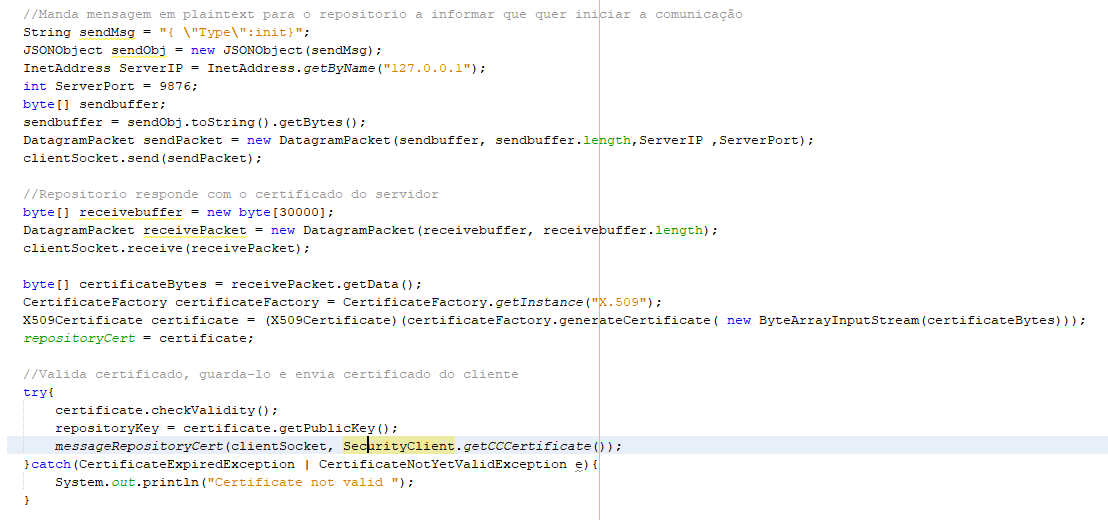
\includegraphics[width=17.0cm]{cert.png}
    \caption{Código relativo á troca de certificados.}
    \label{fig:mesh1}
\end{figure}

\newpage
\subsection{Troca de mensagens cifradas}
Como visto anteriormente a maneira mais rápida de trocar mensagens cifradas é através de encriptação simétrica, para isso é necessário os sistemas acordarem uma chave simétrica, isto ocorre imediatamente após a troca de certificados, é gerada uma chave simétrica com AES, uma vez gerada, é necessário transmitir a mensagem para o seu par, para isso é então assinada e encriptada a chave simétrica, a assinatura é feita com SHA-256 que é um algoritmo de hash ainda não quebrado, tornando-se assim uma das hash functions mais fortes existentes, já a encriptação é feita com RSA com recurso à chave privada sendo depois no seu par verificada a assinatura e decriptada com a chave pública obtida através do certificado previamente trocado. 
\begin{figure}[h]
    \centering
    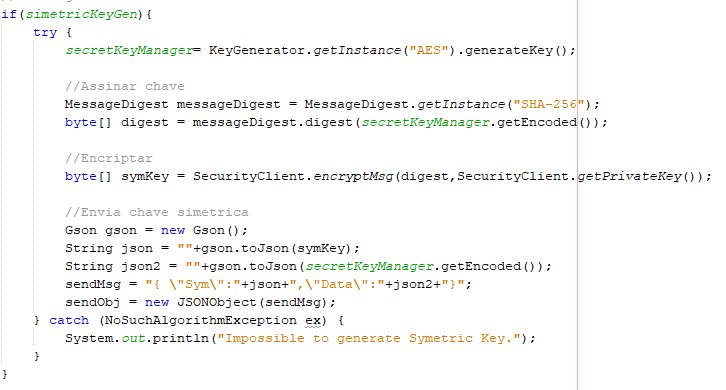
\includegraphics[width=15.0cm]{key.png}
    \caption{Produção de chaves simétricas.}
    \label{fig:mesh1}
\end{figure}

Uma vez com as chaves simétricas acordadas, é usado AES em modo GCM(Galois/Counter Mode), foi escolhido este modo, devido à sua eficiência e performance e também devido a atacar já um novo problema, que é a necessidade de autenticação entre os sistemas.
Apesar de difícil continua a ser possível ataques de brute-force de modo á tentativa de descobrimento da chave simétrica, de modo a reduzir ainda mais essa remota possibilidade, sempre que é encriptada uma mensagem é gerado um novo IV com o recurso a um CSPNRG (cryptographically secure pseudo-random number generator).
\begin{figure}[h]
    \centering
    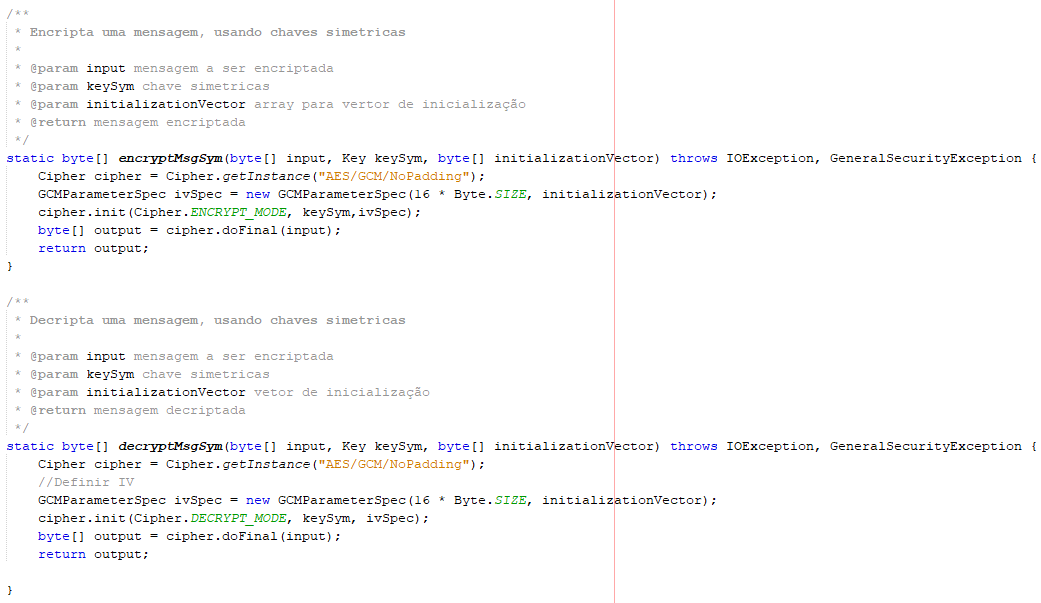
\includegraphics[width=15.0cm]{encrypt.png}
    \caption{Código relativo á troca encriptação e decriptação simétrica.}
    \label{fig:mesh1}
\end{figure}

\vskip 1.5cm
\subsection{Autenticação e controlo de integridade}
Como já vimos anteriormente, a solução que vimos de modo a resolver este problema, foi a utilização de GCM.

\vskip 1.5cm
\subsection{Proteção dos bids até ao final do leilão}
É extremamente importante manter a proteção dos bids até ao final do leilão, para isso quando o cliente deseja fazer um bid, ele procede à assinatura do mesmo e envia para o repositório, que por sua vez envia para o manager, o manager procede à validação do bid e uma vez validado encripta o bid  com uma chave que apenas ele possui, fazendo com que apenas ele possa desencriptar o bid, e devolve o mesmo ao repositório, que por sua vez adicionar à lista de bids do leilão desejado.
No fim do leilão, o repositório procede ao pedido de desencriptação do mesmo pelo manager, o manager faz-lo, e no fim envia ao repositório, que agora já com o bid desencriptado pode verificar a assinatura do bid, garantindo que não houve alguma alteração do mesmo, pois caso tivesse havido, a validação da assinatura falharia.

\vskip 1.5cm
\subsection{Identificação do autor de um bid através do seu CC}
De modo a garantir a identificação e não repudiação de um bid, sempre que um cliente tem de fazer uma bid, ele deve assinar o mesmo, a assinatura é feita com o recurso a SHA256withRSA, sendo usada a chave privada do cliente para assinar, no fim do leilão as bids são verificadas de modo a garantir que não houve qualquer alteração do mesmo, o que nos leva ao seguinte ponto.

\vskip 1.5cm
\subsection{Exposição dos bids necessários no fim de um leilão}
No fim de um leilão devem ser revelados todos os bids e seus autores para o caso de um leilão inglês e apenas os bids para o caso de um leilão cego, no momento da revelação dos bids, são então verificadas todas as assinaturas, sendo todas as assinaturas verificadas com sucesso, são então dependendo do tipo de leilão remetidos para o cliente as informações necessárias.
\begin{figure}[h]
    \centering
    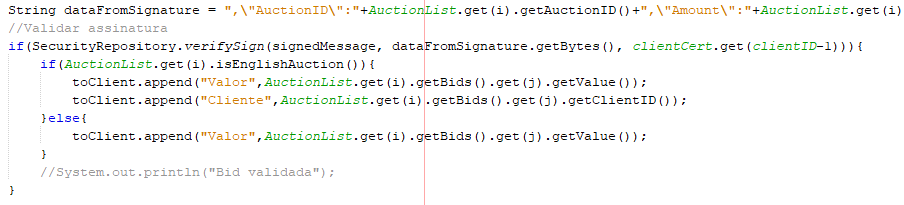
\includegraphics[width=17.0cm]{expose.png}
    \caption{Validação de bids.}
    \label{fig:mesh1}
\end{figure}

\newpage
\vskip 1.5cm
\subsection{Validação dos bids}
A validação dos bids como já visto, é feita pelo manager, esta validação deve ser dinâmica, e inicialmente deveria ser validado o caso de um leilão já ter terminado ou não e as regras básicas relativas a um leilão, que no caso de ser um leilão inglês, apenas exige que o valor da bid seja maior que a maior bid já feita, já no caso de um leilão cego, são todos os valores de bids aceitos.
A parte da validação das regras básicas dos leilões foi concluída com sucesso, no entanto por alguma falta de tempo não foi possível a realização de outras validações, quer sejam relacionadas com o tempo ou com permissões específicas para cada utilizador.
\begin{figure}[h]
    \centering
    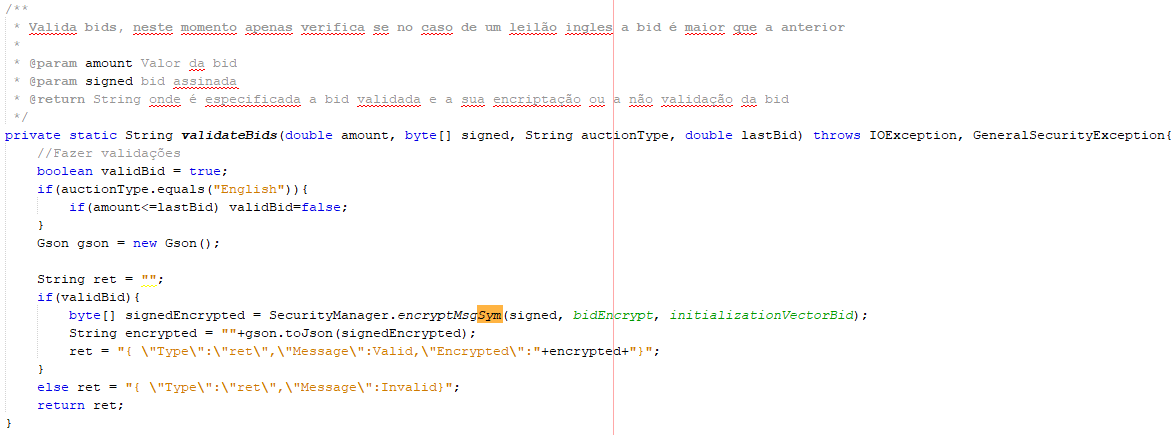
\includegraphics[width=17.0cm]{valid.png}
    \caption{Validação de bids.}
    \label{fig:mesh1}
\end{figure}

\subsection{Modificação de bids validados}
É dada ao manager a possibilidade de encriptação ou desencriptação do bid, no entanto no fim do leilão deve ser possível provar que não houve alteração do mesmo por parte do manager, isto foi de novo feito através de assinaturas, uma bid assinada nunca pode ser alterada, ou será automaticamente invalidada, logo se o manager ou outra qualquer entidade mudar algo acerca da bid, isto faz automaticamente que a assinatura deixe de ser válida o que impossibilita a possibilidade de prova da não alteração dos bids no momento do término de um leilão.

\subsection{Construção de um blockchain por leilão}
Era pedido a construção de uma blockchain para as bids de cada leilão de modo a garantir, que as bids não eram trocadas de ordem, para a implementação disso foi para leilão criada uma lista ligada ordenada, onde no momento da adição de cada bid, era adicionada a hash da lista de bids antes da inserção da nova bid, o que invalida a troca das bids, pois cada nova inserção, vai “selar” inserção prévia.
\begin{figure}[h]
    \centering
    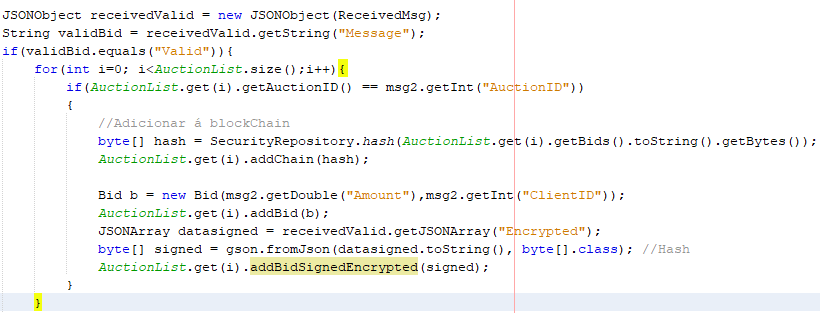
\includegraphics[width=15.0cm]{blockchain.png}
    \caption{Produção da blockchain.}
    \label{fig:mesh1}
\end{figure}

\newpage
\subsection{Criptopuzzles}
Como em todos os sistemas os clientes podem fazer ações desnecessárias que ocupam os servidores, para esse problema foi implementado nas licitações os criptopuzzles. Os criptopuzzles fazem com que os clientes demorem mais tempo a fazer uma licitação com um proof of work. O proof of work consiste em descobrir um número random enviado pelo servidor, quando o cliente descobre o número envia de volta o resultado e caso seja realmente o número gerado, é lhe dado o direito de fazer uma licitação.
\begin{figure}[h]
    \centering
    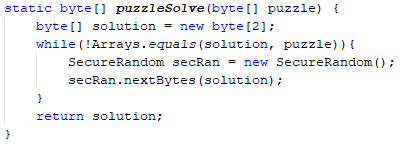
\includegraphics[width=8.0cm]{puzzle.png}
    \caption{Resolução de um puzzle enviado pelo servidor.}
    \label{fig:mesh1}
\end{figure}

\newpage
\vskip 1.5cm
\subsection{Recibos}
Para manter a transparência do leilão é enviado um recibo por cada licitação, isto permite um cliente reclamar se houver algum problema na escolha do vencedor. O servidor ao receber uma licitação e depois da validação dessa, envia o recibo com assinado com a sua chave privada. O cliente pode verificar um recibo com a chave pública do servidor.
\begin{figure}[h]
    \centering
    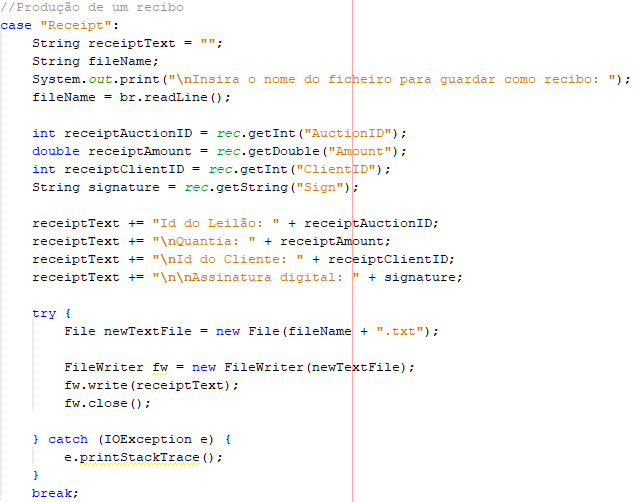
\includegraphics[width=17.0cm]{receipt.png}
    \caption{Produção de um recibo.}
    \label{fig:mesh1}
\end{figure}


\newpage
\section{Conclusão}
Com o desenvolvimento deste projeto foi possível pôr em prática os conhecimentos aprendidos na cadeira de Segurança. O objetivo principal foi concluído com sucesso, procedendo à implementação de políticas de segurança no sistema de gestão de leilões, no entanto devido á pressão de outras cadeiras, não foi possível otimizar o código nem fazer tudo o que havia sido planeado, sendo por exemplo a utilização do tempo uma das coisas que foi deixada para trás.







\end{document}